\documentclass[12pt]{report}
\usepackage[utf8]{inputenc}
\usepackage{setspace}
\usepackage{color}
\usepackage{tikz}
\newcommand\independent{\protect\mathpalette{\protect\independenT}{\perp}}
\def\independenT#1#2{\mathrel{\rlap{$#1#2$}\mkern2mu{#1#2}}}
\usetikzlibrary{shapes,decorations,arrows,calc,arrows.meta,fit,positioning}
\tikzset{
    -Latex,auto,node distance =1 cm and 1 cm,semithick,
    state/.style ={ellipse, draw, minimum width = 0.7 cm},
    point/.style = {circle, draw, inner sep=0.04cm,fill,node contents={}},
    bidirected/.style={Latex-Latex,dashed},
    el/.style = {inner sep=2pt, align=left, sloped}
}
\usepackage{etoolbox}
\usepackage{pdflscape}
\usepackage{geometry}
\usepackage{soul}
\renewcommand{\thesection}{\arabic{section}}
\makeatletter
\setlength{\@fptop}{0pt}
\makeatother
\usepackage[export]{adjustbox}
\newcommand\Tstrut{\rule{0pt}{4ex}}    
\newcommand\Bstrut{\rule[-4ex]{0pt}{0pt}}   % = `bottom' strut
\usepackage{graphicx}
\usepackage{lscape}
\usepackage{lipsum}% http://ctan.org/pkg/lipsum
\usepackage{mdframed}% http://ctan.org/pkg/mdframed
\usepackage{pdflscape}
\usepackage{caption}
\usepackage{rotating}
\usepackage{indentfirst}
\makeatletter
\patchcmd{\thebibliography}{
  \chapter*{\bibname}\@mkboth{\MakeUppercase\bibname}{\MakeUppercase\bibname}}{
  \section{References}}{}{}
\makeatother
\usepackage[round]{natbib}  
\usepackage{geometry}
\usepackage{amsmath}
\usepackage{natbib}
\usepackage{amssymb}
\renewcommand{\bibname}{\vspace{0mm} \large \textbf{References}\vspace*{-10mm}}
\usepackage{titlesec}
\usepackage{amsfonts}
\newcommand{\data}{\textit{Note:} Observations are at the school-by-academic year level. 2020 unique school observations. 8080 total observations. Sample Period: 2014-2017.}
\newcommand{\basereg}{School FE and Year FE included. SE are clustered at the school level.}
\newgeometry{top=1in,bottom=1.5in,left=1in,right=1in}
\title{The Relationship Between Teacher Turnover and Student Performance: Evidence from Pennsylvania's Publicly Funded Schools}
\author{Collin J. Wardius\thanks{Email: collin.wardius@temple.edu. Department of Economics, Temple University.}}
\date{\parbox{\linewidth}{\centering%
  Economics 3598\endgraf\bigskip
  \today}}

\begin{document}

\maketitle

\doublespacing
\section{Introduction}
 
\normalsize \noindent An underexplored determinant of student performance is teacher turnover. Historically, teacher turnover was understood as relatively fixed and due primarily to teacher retirements. Increasingly though, turnover is due to new teachers leaving the profession. As is noted in \cite{watlington}, 50\% of new teachers leave the profession after their first five years of teaching. The average number of teachers of any experience level leaving the profession is also steadily rising. As is documented in \cite{hammond}, 5.1\% of teachers left the profession in 1994, whereas 8.4\% left in 2005. While a three percentage point increase may seem trivial, this amounts to approximately 90,000 positions. Given this trend, examining the effects of teacher turnover on students is of vital public interest. \newline
\indent Data compiled by the Pennsylvania Department of Education (PDE) provide an opportunity to study whether teacher turnover is causally related to student performance. Across model specifications, I find that teacher turnover has a negative and statistically significant effect on student performance with the most pronounced effect in math performance. \\ 
\indent These findings suggest that teacher turnover is something policymakers should be concerned with reducing. Moreover, as teacher turnover is more concentrated in impoverished areas, like Philadelphia county (see \cite{phl}), reducing turnover should be examined as a means to reduce learning inequities.
\section{Literature Review}
\normalsize \noindent Two types of teacher turnover effects, as outlined in \cite{ronfeldt}, guide the following theoretical discussion: compositional effects and disruptive effects. 
\\
\indent Compositional effects are those that affect faculty quality at a given school and can be either positive or negative. If less effective teachers leave and more effective teachers subsequently join the teaching faculty, then the aggregate skill of the teaching faculty increases, a positive compositional effect. Alternatively, if effective teachers migrate from, say, lower performing schools, then the aggregate skill of the teaching faculty at those schools decreases, a negative compositional effect. \\
\indent Disruptive effects are those that impact the general organization and allocation of resources within a school. Consider the following disruptive effects of teacher turnover. One, teacher turnover involves the hiring and training of new teachers; both processes are time consuming and costly. Two, constant turnover implies that students cannot build solid relationships with their teachers. Three, remaining teachers may feel uncomfortable and isolated if there is continual faculty turnover. Four, new teachers may implement instructional programs in a manner inconsistent with senior faculty. \\
\indent While it is difficult to measure in dollars compositional turnover effects, there have been efforts to measure disruptive turnover effects. \cite{barnes} examines teacher turnover costs across different geographies and found that the cost to replace teachers is higher in more urban geographies. Specifically, turnover costs are \$10,000 in a suburban North Carolina county per teacher, \$15,325 per teacher in Milwaukee, WI, and \$26,502 in Chicago, IL. \\
\indent There are two important implications of this discussion. One, schools would prefer no turnover to turnover all else equal because of negative disruptive effects. Two, teacher turnover is not necessarily harmful and could, in fact, be beneficial conditional on overall teacher quality increasing and outweighing the disruptive effects of teacher turnover. Indeed, there is broadening literature, including \cite{staiger}, on the positive effects of retaining effective teachers, and dismissing ineffective teachers, on student performance. Empirical studies also show that there is potential for positive compositional effects outweighing disruptive effects. For example, \cite{adnot} examines the performance-assessment and incentive system IMPACT implemented in the District of Columbia Public Schools. Due to IMPACT, a significant portion of ineffective D.C. public school teachers were purposefully compelled to leave. In their sample, \cite{adnot} finds that teacher turnover does not have a statistically significant effect on student performance. This implies that the negative disruptive effects of teacher turnover were balanced by the positive compositional effects of IMPACT that aimed to dismiss ineffective teachers exclusively.
\\
\indent Under more general conditions, however, empirical studies suggest a negative causal relationship between teacher turnover and student outcomes. For example, \cite{ronfeldt} finds that teacher turnover is associated with a decrease in student performance on math and language arts assessments among fourth and fifth grade students in New York City. \\
\indent This paper adds to the literature in three ways. First, it employs a unique instrumental variable identification strategy that addresses the simultaneity bias inherent in measuring the effect of teacher turnover on student performance. Second, it assesses whether the effects of teacher turnover are robust from New York to Pennsylvania. Third, it finds evidence of a quadratic relationship between teacher turnover and student performance. 

\section{Model}
\noindent Teacher turnover is measured using the method from \cite{ronfeldt} adapted to the school-academic year level of aggregation:
\begin{equation}
d_{st} = m_{st} / n_{st}
\end{equation}
\noindent In words, turnover at school $s$ in academic year $t$ is calculated through taking the total number of new teachers in the current academic year, $m_{st}$, over the total number of teachers in the current academic year $n_{st}$. I will refer to this measure of teacher turnover as \textit{proportion new} throughout the rest of this paper and interchangeably use the terms proportion new and teacher turnover. \\
\indent \cite{ronfeldt} discusses other methods to measure teacher turnover. Namely, a measure which they call ``lagged attrition" defined as the number of teachers that were teaching at school $s$ in period $t-1$, but were not teaching at school $s$ in period $t$. How teacher turnover is measured should not matter causally; therefore, for future versions of this paper, I plan to rerun major analyses from the results section of this paper with the lagged attrition measure.  \\
\indent To study the relationship between student performance and proportion new, I estimate the following equation.
\begin{equation}
y_{st} = d_{st}\gamma + x_{st}'\beta + \lambda_s + \delta_t + \epsilon_{st}
\end{equation}
where $y_{st}$ is student performance, $d_{st}$ is proportion new, $x_{st}$ is a vector of controls, $\lambda_s$ is school fixed effects, and $\delta_t$ is academic year fixed effects.  \\
\indent As this is a school fixed effects model, $\gamma$ is estimated using within school variation in teacher turnover. School fixed effects effectively controls for unobserved, time-invariant features of schools, like location, whether the school is a public school or a charter school, aggregate student ability, and aggregate teacher quality. Academic year fixed effects control for time trends in scores. \\ 
\indent Now, for $\hat{\gamma}$ to have a causal interpretation, the conditional independence assumption: $y_{std}\independent d_{st}|x'_{st},\lambda_s,\delta_t$, must be satisfied. Note that $y_{std}$ is potential student performance for school $s$ in time period $t$ for level $d$ of teacher turnover. This assumption implies that conditional on our controls, school fixed effects, and year fixed effects, a school's level of teacher turnover is as good as randomly assigned. To satisfy this condition, I include controls for certain characteristics of schools that vary over time and impact student performance: teachers per student at the the school level, administrators per student at the school level, and county median income. \\
\indent Even with these controls, it is unlikely that the conditional independence assumption is satisfied. For example, suppose a school endogenously implements a new remedial policy that requires students to see a math specialist should they fall below some minimal level of performance. This is an omitted variable bias problem since we cannot control for such policy changes. So if one was to estimate $\gamma$ from the above equation, one would na\"{i}vely estimate 
\begin{equation}
\hat{\gamma}=\xi+\tau\sigma
\end{equation}
\noindent In words, $\hat{\gamma}$ is equal to the true effect of teacher turnover on student performance, $\xi$, plus an error term, $\tau\sigma$. The error term consists of $\tau$: the effect of the remedial policy on student performance, multiplied by $\sigma$: the effect of the remedial policy on proportion new. Though we cannot estimate this error term, we can make some reasonable assumptions about its nature. It is likely that $\tau>0$ as the policy helps marginal students perform better. It is also likely that $\sigma>0$ since such a policy would require the hiring of a new math specialist teacher. Therefore, our estimate, $\hat{\gamma}$, will be ``too positive" in the sense that $\hat\gamma >\gamma$. Now, the magnitude by which our estimate is biased is up for debate and depends on how significant one expects the error term is. Furthermore, our estimate of $\gamma$ could be impacted by other variables that are less obvious than school policy changes yet still affect student performance. \\
\indent In addition to the omitted variable bias problem, there is also a simultaneity issue in this model. Low student performance could cause a higher proportion of new teachers through two channels. One, teachers think that their students are not able to be taught and consequently quit teaching or move to a different school, requiring new teachers to be hired on. Two, the school hires on additional teachers to give students more individualized attention. Hence, the data generating process for both proportion new and for student performance is the same. This implies that $\mathbb{E}[d_{st}\epsilon_{st}|x_{st},\lambda_s,\delta_t]\not=0$ and the conditional independence assumption is violated. \\
\indent To address both the omitted variable and the simultaneity problems, I employ an instrumental variable (IV) estimation strategy using expenditures per student as an instrument for proportion new. In the first stage, I estimate the following equation
\begin{equation}
d_{st} = z_{st}\rho + x_{st}'\beta + \lambda_s + \delta_t + e_{st}
\end{equation}
\noindent where $z_{st}$ is expenditures per student. After estimating the first stage, I then estimate the second stage equation
\begin{equation}
y_{st} = \hat{d}_{st}\gamma + x_{st}'\beta + \lambda_s + \delta_t + \epsilon_{st}
\end{equation}
\noindent where I plug in estimated values from the first stage for proportion new as opposed to sample values. \\
\indent Under this identification strategy, variation in expenditures per student within school causes exogenous variation in proportion new within school. This exogenous variation is then used to estimate the effect of proportion new on student performance (see Figure 1). \noindent Notice that the expenditures per student instrument solves both of the problems identified with estimating $(1)$ na\"{i}vely. Namely, since changes in expenditures per student are not influenced by school learning policy changes and potentially other unobserved variables, the omitted variable bias problem is avoided. Furthermore, while changes in proportion new and student performance are simultaneously determined, changes in expenditures are not determined by either variable.
\begin{figure}[h!]
\begin{center}
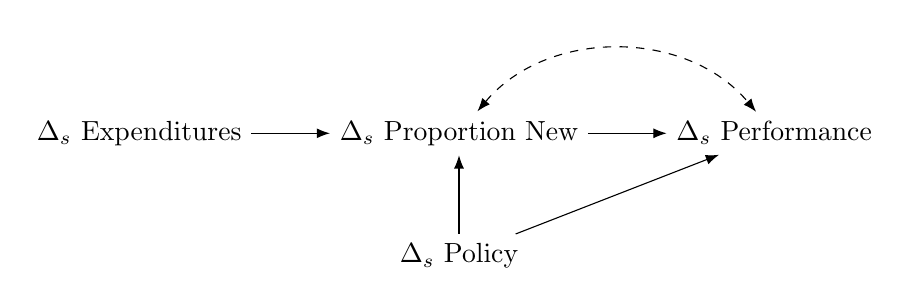
\begin{tikzpicture}
    \node (1) at (0,0) {$\Delta_s$ Expenditures};
    \node (2) [right = of 1] {$\Delta_s$ Proportion New};
    \node (3) [right = of 2] {$\Delta_s$ Performance};
    \node (4) [below = of 2] {$\Delta_s$ Policy};

    \path (1) edge (2);
    \path (2) edge (3);
    \path[bidirected] (2) edge[bend left=50]  (3);
    \path (4) edge (3);
    \path (4) edge (2);
\end{tikzpicture}
\end{center}
\caption{Causal Chain with Expend. per Student IV}
\end{figure}

\indent For the instrument to be valid, it must satisfy the following two conditions:

\singlespacing
\begin{enumerate}
    \item Relevance: $\mathbb{E}[z_{st}d_{st}]\not=0$.
    \item Exogeneity: $\mathbb{E}[z_{st}\epsilon_{st}]=0$.
\end{enumerate}

\doublespacing
\noindent Theoretically, it is unclear whether the relevance condition is satisfied. Expenditures per student increases the number of teachers a school can hire thereby increasing proportion new. However, higher expenditures per student likely implies that there are more resources to support teachers, encouraging them to stay. I empirically test for relevance through estimating the first stage in the results portion of this paper. Such results suggest that the instrument is indeed relevant. \\
\indent Now, we examine the exogeneity condition. Are there any unobserved variables that are correlated with expenditures per student that also impact student performance? This requires an examination of how public schools are funded in Pennsylvania. Almost all of a school's funding comes from three sources: local taxes, the state, and the federal government with local taxes having the highest contribution on average. Since school funding is relatively decentralized in Pennsylvania, there are considerable disparities among expenditures per student (see \cite{funding}). Specifically, wealthier areas have higher property taxes and can therefore heavily fund schools whereas more impoverished areas have lower property taxes and cannot heavily fund schools. Of course, state and federal funding helps to smooth the funding gap between localities but this is often insufficient (again, see \cite{funding}). This is an apparent threat to the exogeneity condition. Expenditures per student is correlated with local wealth and local wealth likely increases student performance. However, we are able to control for this (roughly) through including county median as a control variable. One could also argue that wealthier parents more closely monitor their children to ensure that their school work gets done, thus boosting performance. There is no obvious control for such parenting. Recall though that school fixed effects are included in the model. So, if parenting at a given school is constant from year to year, this effect will be differenced out.\\ 
\indent The last exogeneity concern I will address is that school performance and funding are simultaneously determined. Consider that in Pennsylvania schools can apply for School Improvement Grants (SIGs): competitive grants that allow low-performance schools to acquire more state-funding. This is a problem since there is no control for a school's receiving such grants with the current data. Therefore, the extent to which the instrument is exogenous is determined by the extent to which state and local governments in Pennsylvania are sensitive to the poor performance of their schools. Such a question requires further research.\\
\indent In this paper, I also provide evidence that teacher turnover has a quadratic relationship with student performance modeled by the following equation:
\begin{equation}
y_{st} = {d}_{st}\psi + (d_{st})^2\zeta + x_{st}'\beta + \lambda_s + \delta_t + \epsilon_{st}
\end{equation} 
I estimate the above school fixed effects model. Additionally, I slightly modify the IV identification strategy from before since there are now two endogenous variable: $d_{st}$ and $d_{st}^2$. First, I estimate 
\begin{equation}
d^2_{st} = z_{st}\rho + x_{st}'\beta + \lambda_s + \delta_t + e_{st}
\end{equation}
I take the fitted values obtained from (7), label them $r_{st}$, along with our original instrument $z_{st}$ to estimate the following two equations\footnote{Assuming that $z_{st}$ is exogenous, $r_{st}$ is a function of exogenous variables and is therefore itself exogenous and can be used as an IV. See \cite{wooldridge}.}
\begin{align}
d_{st} & = z_{st}\rho + r_{st}\omega + x_{st}'\beta + \lambda_s + \delta_t + e_{st} \\
d^2_{st} & = z_{st}\rho + r_{st}\omega + x_{st}'\beta + \lambda_s + \delta_t + e_{st}
\end{align}
\noindent I then estimate the following second stage equation:
\begin{equation}
y_{st} = \hat{d}_{st}\gamma + \widehat{(d_{st})^2}\zeta + x_{st}'\beta + \lambda_s + \delta_t + \epsilon_{st}
\end{equation} 
\noindent Note well that notation here is tricky. In the second stage, I am expressly \textit{not} using the square of the fitted values from $(8)$ but rather the fitted values obtained from $(9)$. In general, $\widehat{(d_{st})^2}\not = (\hat{d_{st}})^2$. Assuming that our original instrument, $z_{st}$, is valid, then $r_{st}$ is also valid. \\
\indent A quadratic relationship seems reasonable since low turnover likely aids student performance as older, less effective teachers retire and younger, more passionate teachers join the faculty. However, we would expect student outcomes to decrease as turnover becomes large since the disruptive effects of such turnover likely compound. For example, it is likely easy for a school to hire on new teachers if only a few leave. However, if many leave at one time, many more resources must be allocated to hiring and training new teachers, trading off with other services to students. In terms of (6), we would expect $\psi>0$ and $\zeta < 0$.
\section{Data}
\normalsize \noindent I merge together the following four distinct PDE datasets to construct my final data set. One, Pennsylvania System of School Assessment (PSSA) data at the school-academic year level are available from academic year 2014 to academic year 2018. Two, teacher data at the teacher-academic year level document a teacher's school and teaching assignment, along with a range of variables useful for tracking teachers over time, namely salary, level of education, and years of experience. Three, student enrollment data are available at the school-academic year level and at the school district-academic year level. Four, expenditure data are available at the school district-academic year level for all years excluding academic year 2018. Since expenditure data is not available in 2018, my analysis will be limited to years 2014 through 2017. \\
\indent There are elements of my constructing the proportion new measure of teacher turnover that are of note. I drop all teachers who are listed as subcontracted, inactive in teaching status, part time, or missing key identifying information (name or school assignment). Teachers are counted as new when their name first appears in the data within a particular school. This method of identifying new teachers is rather coarse and is potentially prone to a number of errors: one, if a teacher changes their name, a teacher would be counted as new within a school twice. Two, it relies on schools consistently reporting the proper names of all their teachers. The issues described here are only important if either the frequency at which teachers change their names or the frequency of schools misreporting their teachers' names is endogenous to the school. One could perhaps tell a story about how low-performing schools are more disorganized and are consequently more prone to reporting teachers' names incorrectly. Whether or not this story is valid is hard to test. Figure 4 in the appendix presents the distribution of average proportion new by school. It has a similiar shape to the distribution of proportion new by school in \cite{ronfeldt}, albeit with a lower mean. The relatively lower mean of my proportion new measure is likely a consequence of measuring turnover at the school level as opposed to the grade level as \cite{ronfeldt} does. 
\\
\indent Scores from the PSSA serve as a measure of student performance. Students enrolled in public schools and publicly funded charter schools take the PSSAs in math and English at each grade level from grade three to grade eight. Additionally, students take the PSSA in science during grades four and eight. Based on a student's score on a particular assessment, a student's performance is classified lexically as advanced, proficient, basic, or below basic. Students scoring in either the basic or below basic categories are typically prescribed remedial support and scoring on the PSSA influences a student's individualized education plan (IEP\footnote{IEPs are plans for students with special needs.})\nocite{pssa}. The PSSA is designed to inform students, parents, educators, students, citizens, and legislators on student performance.\footnote{See Pennsylvania Department of Education (2012) \nocite{pssa} for further information on the goals of the PSSA.} 
\\
\indent I construct measures of school-grade performance through summing the proportion of students who achieved proficient or advanced on each PSSA for each school. This implies that there are 14 school-grade performance variables as there are six tests in math, six tests in English, and two tests in science. 
\\
\indent I construct an aggregate measure of student performance at the school level. By school, I take the average percentage of students scoring advanced or proficient across all PSSA subject areas administered at that school and across all grades. Notably, using this sort of measure will not allow us to capture whether there are different effects of teacher turnover by grade or different effects of teacher turnover by subject area. Now, one might be worried that such a measure will be distorted since different schools take different PSSAs. For example, middle schools will only take PSSAs for grades six through eight. As will be shown, scores on math PSSAs in grades five through eight are significantly lower than in earlier grades. Therefore, one would expect middle schools to have lower aggregate performance than primary schools. However, recall that only within school variation is used to estimate the parameters of my models. Therefore, distortions from school to school on this measure are inconsequential for estimation purposes. A different concern is that if a school takes different tests over time, that would impact the aggregate performance measure from year to year, but would not be representative of a true change in student ability. For example, if Kennett Middle School did not report PSSA math performance in 2014 and then reported PSSA math performance in 2015, that would likely heavily impact the aggregate performance measure for 2015 relative to 2014 in a way that is not representative of a change in students' ability. I deal with this problem through dropping all schools that do not take the same tests throughout the sample period. \\
\indent I construct three, subject-specific aggregate school measures of student performance. These are constructed very similarly to the measure described above except instead of averaging over all the PSSAs students at a school take, I average over subjects individually. For example, if some school reported statistics for Math PSSAs for grades six through eight, then the aggregate math performance measure would be the average number of students scoring advanced or proficient across all math PSSAs. \\
\indent I make a number of modifications to the raw PDE data. First, I drop all schools that do not have PSSA scores. Second, I drop all schools that are not in the data for the four years of study. These cases are relatively few and are issues of data quality or schools closing. These steps create a strongly balanced panel data set. I think it is sensible to exclude schools that are closing from the analysis as those schools face fundamentally different circumstances than other schools which could distort estimates. I also drop all schools from the sample that did not take the same tests from year to year. Finally, I drop from the sample any schools where proportion new was greater than 50\%. Such schools constitute approximately 3.6\% of the schools sampled and seem to be cases of name reporting issues. All analyses have been rerun without dropping these observations of high turnover; they yield qualitatively similar results and are available upon request. \\
\indent In addition to PDE data, I merge on county median income from the American Community Survey. Notably, there are missing observations for 14 of Pennsylvania's 67 counties in the year of 2015. I interpolate these values by taking the average between 2014 median income and 2016 median income for said counties.  \\
\indent Now, I discuss some limitations of the data. One, turnover is measured at the school level, rather than at the school-grade level. One could argue that, for example, teacher turnover in first grade minimally impacts student performance in fifth grade, leading to imprecise estimates of the effect of turnover on school-grade performance measures. This sentiment is roughly correct; however, I think turnover does likely have some systemic effect on schools. As was discussed prior, turnover potentially leads to inconsistent curriculum implementations, isolates remaining faculty, and requires school resources to replace leaving teachers that likely trade off with resources for student programs.\\
\indent Two, there are some variables that are not as precise as one would wish. For example, the only given geographic feature of a school is county. This prohibits merging on ACS data at some more granular census geography (like tract). Given more time, I would attempt to map schools to census tracts and merge on ACS data at the tract level.\\
\indent Three, the PDE does not provide an identifier to track teachers through time. This is why I rely on a teacher's name to flag them as new to a school. Of course, this method is prone to issues as I discuss earlier in this paper.\\
\indent See Table 1 for summary statistics for the data set.\footnote{See Figures 6-8 to see the distributions of the grade-level performance variables.} Of note is a noticeable trend downward in Math scores as grade level increases. Indeed, this trend is documented in \cite{lancaster}. \\
\indent I also characterize the data geographically in Figures 3 and 4 of the appendix. Figure 3 plots the locations of the $2,020$ schools in the sample. Figure 4 plots average teacher turnover by county. We see that turnover is particularly high in urban counties like Philadelphia. This is consistent with stories in the popular press like \cite{phl}.

\begin{table}[h!]\centering
\def\sym#1{\ifmmode^{#1}\else\(^{#1}\)\fi}
\caption{Summary Statistics, Pennsylvania Department of Education and American Community Survey Data from 2014 to 2017.}
\begin{tabular}{l*{1}{cccc}}
\hline\hline

                    &  Mean&          SD&         Min&         Max\\
\hline
\textit{School \& County Features} \\
\hline
\rule{0pt}{4ex}Proportion New (\%)  &        9.88&        9.52&        0.00&       50.00\\
Teacher to Student Ratio (\%)&        7.49&        1.63&        2.54&       28.70\\
Admin. to Student Ratio (\%)&        0.31&        0.18&        0.00&        2.60\\
Expend. per Student (\$1,000)&       18.20&        4.24&        8.38&       60.49\\
County Median Income (\$1,000)&       28.03&        4.95&       14.88&       40.15\\
\hline
\textit{Performance Measures} \\
\hline
\rule{0pt}{4ex}Math Grade 3        &       54.52&       21.75&        0.00&      100.00\\
Math Grade 4        &       46.30&       21.84&        0.00&      100.00\\
Math Grade 5        &       44.36&       22.03&        0.00&       98.30\\
Math Grade 6        &       38.88&       20.63&        0.00&      100.00\\
Math Grade 7        &       33.03&       18.85&        0.00&       93.30\\
Math Grade 8        &       27.96&       17.38&        0.00&       85.10\\
Science Grade 4     &       76.92&       19.14&        7.00&      100.00\\
Science Grade 8     &       52.38&       21.61&        0.00&      100.00\\
English Grade 3     &       64.32&       19.58&        3.70&      100.00\\
English Grade 4     &       60.31&       20.54&        1.40&      100.00\\
English Grade 5     &       60.76&       21.09&        0.00&      100.00\\
English Grade 6     &       60.70&       20.48&        0.00&      100.00\\
English Grade 7     &       57.07&       20.13&        1.90&      100.00\\
English Grade 8     &       56.22&       19.97&        0.00&      100.00\\
Agg. Math Performance    &       45.31&       20.59&        0.00&       97.80\\
Agg. Science Performance &       70.76&       21.28&        1.00&      100.00\\
Agg. English Performance &       62.53&       18.51&        4.33&      100.00\\
Agg. School Performance&       56.35&       18.98&        2.27&       97.59\\
\hline\hline
\end{tabular}
\caption*{\textit{Note:} Data at school-by-academic year level. 2,020 schools. 8,080 observations.}
\end{table}
\clearpage
\section{Results}
\noindent I split the results section of this paper into three distinct subsections. In the first subsection, I provide evidence that the instrument, expenditures per student, is relevant. In the second subsection, I present aggregate findings on the linear and quadratic relationship between teacher turnover and student performance. In the third subsection, I examine how the effect of teacher turnover varies by geography, by income level, and by subject. I also provide suggestive evidence that teacher turnover has an especially pernicious effect on low-performing schools.

\subsection{Instrument Validity}
\noindent In Table 2, I provide evidence of the relevance of expenditures per student as an instrument. Three items from this table are of note. First and most importantly, estimation of the first stage shows that the instrument is relevant. This is evidenced both by the instrument having a statistically significant effect on proportion new and by the F statistic being 1,244. When one examines instrument relevance, one looks for an F statistic greater than ten, a rule of thumb from \cite{yogo}. Two, the effect of expenditures per student on proportion new is moderately large as a one thousand dollar increase in expenditures per student increase proportion new by .17 percentage points relative to a mean of proportion new of 9.88 as is seen in Table 1. Three, the R-squared for this model is quite high as 51\% of the within-school variation in proportion new is explained by this model.

\begin{table}[!htb]
\caption{First Stage Regression of Proportion New on Expenditures per Student}
    \centering
\begin{tabular}{lc}
\hline\hline
 & (1) \\
VARIABLES & School FE \\ \hline
 &  \\
Expend. per Student (\$1,000) & 0.17*** \\
 & (0.06) \\
Teacher to Student Ratio (\%) & 1.77*** \\
 & (0.20) \\
Administrator to Student Ratio (\%) & -1.37 \\
 & (1.11) \\
County Median Income (\$1,000) & 0.05 \\
 & (0.29) \\
 &  \\
Observations & 8,080 \\
Number of Schools & 2,020 \\
R-squared & 0.51 \\
 F-test & 1,244 \\
 Mean of Proportion New & 9.88\\\hline\hline
\multicolumn{2}{c}{ Robust standard errors in parentheses} \\
\multicolumn{2}{c}{ *** p$<$0.01, ** p$<$0.05, * p$<$0.1} \\
\end{tabular}

\end{table}
\newpage
\subsection{Aggregate Findings}

\noindent \normalsize In Table 3, I report estimates for the effect of proportion new on the aggregate school student performance measure. Four items are of note. One, in both the School FE and in the School FE, IV model, we reject the null hypothesis that proportion new does not have a statistically significant effect on student performance at the one percent and ten percent significance levels respectively. Two, the analysis of omitted variable bias from the model section of this paper is apparently correct. In the School FE model, we see that the effect of proportion new on student performance is much smaller in magnitude as compared to the effect estimated from the School FE, IV model. This is helpful since the the effect of teacher turnover estimated from the School FE model serves as an upper bound on the effect of teacher turnover on student performance. Therefore, even if one doubts the IV identification strategy, the School FE model provides confidence that teacher turnover indeed has a negative and statistically significant effect on student performance. Three, there is no natural interpretation for R-squared in IV models; therefore, it is missing from the table. Four, county median income does not have a statistically significant effect on student performance. I suspect that this is a consequence of there being little variation in this variable over the sample period. I have included Figure 10 in the appendix as evidence of this explanation.\\
\indent In Table 4, I provide evidence of a quadratic relationship between proportion new and student performance. Two items are of note. One, both proportion new and $(\text{proportion new})^2$ are statistically significant at the $.01$ percent and $.05$ percent significance levels respectively in the School FE, IV model. In contrast, the School FE model suggests that the quadratic term is not statistically significant. Two, the  School FE, IV model provides evidence for our hypothesis that there is some optimal level of teacher turnover. Indeed, we can solve for it. Through plugging in our estimates from Table 4 into (6), we obtain 
\begin{equation}
y_{st} = d_{st}(.38) + (d_{st})^2(-.02) + x_{st}'\beta + \lambda_s + \delta_t + \epsilon_{st}
\end{equation}
\noindent Now, we solve the problem:
\begin{equation}
\max_{d_{st}}\{d_{st}(.38) + (d_{st})^2(-.02) + x_{st}'\beta + \lambda_s + \delta_t + \epsilon_{st}\}
\end{equation}
\noindent which yields the following first order condition for an interior solution 
\begin{equation}
0 = .38 + (-.04)(d_{st}^*) 
\end{equation}
\noindent solving for $d_{st}^*$ yields $d_{st}^*\approx 24.47$\%. This estimate of optimal proportion new seems higher than intuition would suggest. For our sample specifically, this implies that approximately 92\% of the observations have a proportion of new teachers that is below the optimum and 8\% of the sample have a proportion of new teachers that is above the optimum.

\begin{table}[!htb]
\caption{Relationship Between Proportion New and Aggregate Student Performance}
    \centering
\begin{tabular}{lcc}
\hline\hline
 & (1) & (2) \\
 &  & School FE \\
VARIABLES & School FE & IV \\ \hline
 &  &  \\
Proportion New (\%) & -0.05*** & -0.31* \\
 & (0.01) & (0.16) \\
Teacher to Student Ratio (\%) & 0.53*** & 1.00*** \\
 & (0.09) & (0.32) \\
Administrator to Student Ratio (\%) & 0.00 & -0.35 \\
 & (0.57) & (0.67) \\
County Median Income (\$1,000) & 0.21 & 0.23 \\
 & (0.20) & (0.21) \\
 &  &  \\
Observations & 8,080 & 8,080 \\
R-squared & 0.05 &  \\
Number of Schools & 2,020 & 2,020 \\ 
Mean of Agg. School Performance & 56.35 & 56.35\\ \hline\hline
\multicolumn{3}{c}{ Robust standard errors in parentheses} \\
\multicolumn{3}{c}{ *** p$<$0.01, ** p$<$0.05, * p$<$0.1} \\
\end{tabular}

\end{table}
\clearpage
\begin{table}[!htb]
\caption{Quadratic Relationship Between Proportion New and Agg. Student Performance}
    \centering
\begin{tabular}{lcc}
\hline\hline
 & (1) & (2) \\
 &  & School FE \\
VARIABLES & School FE & IV \\ \hline
 &  &  \\
Proportion New (\%) & -0.06*** & 0.38*** \\
 & (0.02) & (0.14) \\
$(\text{Proportion New})^2$ & 0.00 & -0.02** \\
 & (0.00) & (0.01) \\
Teacher to Student Ratio (\%) & 0.53*** & 0.65*** \\
 & (0.09) & (0.21) \\
Administrator to Student Ratio (\%) & 0.01 & -0.33 \\
 & (0.57) & (0.66) \\
County Median Income (\$1,000) & 0.21 & 0.32 \\
 & (0.20) & (0.22) \\
 &  &  \\
Observations & 8,080 & 8,080 \\
R-squared & 0.05 &  \\
 Number of Schools & 2,020 & 2,020 \\
 Mean of Agg. School Performance & 56.35 & 56.35\\\hline\hline
\multicolumn{3}{c}{ Robust standard errors in parentheses} \\
\multicolumn{3}{c}{ *** p$<$0.01, ** p$<$0.05, * p$<$0.1} \\
\end{tabular}

\end{table}

\subsection{Heterogeneity Analyses}
\noindent Table 5 demonstrates significant heterogeneity among subjects in how teacher turnover affects student performance. The first three columns are estimated in the fashion of the School FE model from before and the last three in the fashion of the School FE, IV model from before. Of particular interest is the effect on math performance which is rather large and statistically significant regardless of regression specification. This result stands in contrast to the effect of teacher turnover on English and Science performance where the estimated effect is not statistically significant across regression specifications. \\
\indent I suspect that the observed differential effects by subject are a function of how teacher turnover disrupts curriculum implementation. Math, in contrast to other subjects, builds heavily upon itself and requires students to master basic topics to move on to more advanced ones. The disruption endemic to teacher turnover likely prevents students from mastering the basic of mathematics and therefore struggling with more advanced topics.\\
\begin{table}[!htb]
\caption{Relationship Between Proportion of New Teachers and Performance by Subject}
    \centering
\begin{tabular}{lcccccc}
\hline\hline 
 & (1) & (2) & (3) & (4) & (5) & (6) \\
VARIABLES & Math  & Eng.  & Sci.  & Math IV & Eng. IV & Sci. IV \\ \hline
 &  &  &  &  &  &  \\
Proportion New (\%) & -0.07*** & -0.04*** & -0.03** & -0.45** & -0.26 & 0.01 \\
 & (0.01) & (0.01) & (0.01) & (0.22) & (0.19) & (0.21) \\
Teacher to Student Ratio (\%) & 0.49*** & 0.51*** & 0.71*** & 1.19*** & 0.91** & 0.64 \\
 & (0.12) & (0.11) & (0.16) & (0.43) & (0.37) & (0.41) \\
Admin. to Student Ratio (\%) & -0.18 & 0.39 & -0.75 & -0.70 & 0.09 & -0.69 \\
 & (0.76) & (0.64) & (1.02) & (0.91) & (0.72) & (1.05) \\
County Median Income (\$1,000) & 0.48* & -0.18 & 0.50* & 0.51* & -0.16 & 0.49* \\
 & (0.26) & (0.23) & (0.29) & (0.28) & (0.24) & (0.29) \\
 &  &  &  &  &  &  \\
Observations & 8,080 & 8,080 & 7,654 & 8,080 & 8,080 & 7,654 \\
R-squared & 0.12 & 0.04 & 0.08 &  &  &  \\
 Number of Schools & 2,020 & 2,020 & 1,916 & 2,020 & 2,020 & 1,916 \\
 Mean of Subj. Agg. Perform. & 45.31 & 62.53 & 70.76& 45.31 & 62.53 & 70.76\\
 \hline\hline
\multicolumn{7}{c}{ Robust standard errors in parentheses} \\
\multicolumn{7}{c}{ *** p$<$0.01, ** p$<$0.05, * p$<$0.1} \\
\end{tabular}




\end{table}
\clearpage
\indent In Table 6 of the appendix, I examine the effect of teacher turnover in urban vs. suburban counties. Unfortunately, the estimates are too imprecise to draw any conclusions.\\
\indent In Table 7 of the appendix, I examine the effect of teacher turnover in the 5 highest income counties as compared to the 5 lowest income counties. Again, the estimates are too imprecise to draw any conclusions. I believe that the results observed in tables 6 and 7 are a consequence of relatively small sample sizes.\\
\indent In Tables 8-10 of the appendix, I estimate the effect of changes in proportion new on each of the individual PSSA performance measures. The intent of this exercise is to tease out whether turnover is especially harmful to performance in certain grades. Our estimates are again too imprecise to draw any real conclusions. This lends credence to the idea discussed in the data section of this paper that grade level turnover data is likely required to estimate changes in performance for particular grades.\\
\indent In Figure 2, I chart the estimated effect of changes in proportion new on aggregate student performance and their corresponding 95\% confidence intervals over quantiles .05 to .95. Here is how to interpret this chart. At the .2 quantile, we see that the effect of proportion new on aggregate student performance is approximately .6. This means that at the .2 quantile of aggregate student performance, a one percentage point increase in proportion new decreases the expected aggregate percentage of students scoring advanced or proficient across all PSSAs at a given school by .6 percentage points. \\
\indent There are two items to note from Figure 2. One, the chart suggests that the effect of teacher turnover is most pronounced at schools below the .4 quantile. I.e., schools that have relatively low performance are those that are most hurt by teacher turnover. Two, this evidence is merely suggestive. I estimated a simple pooled linear quantile regression model using the usual controls to generate this graph. Under such a model, the conditional independence assumption must be satisfied for estimates to have a causal interpretation; this is unlikely given that we cannot include school fixed effects. 

\begin{figure}[!htb]
    \centering
      \caption{The Effect of Proportion New on Aggregate Student Achievement by Quantile}
    \includegraphics[frame, scale=0.25]{tt_effect_by_quantile.png}
    \label{fig:my_label}
\end{figure}
% aggregate performance.31 * 9.52
%
\section{Conclusion}
\noindent Teacher turnover has a negative and statistically significant effect on student performance. Evidence of this is consistent across model specifications. At a minimum then, this paper verifies findings from \cite{ronfeldt} and has shown that turnover's deleterious effects are common between Pennsylvania and New York.\\
\indent Aside from statistical significance, there is the question of actual significance. I.e., is the estimated effect of teacher turnover meaningful in the real world? The answer to this question seems to be yes. From Table 3, we see that increasing teacher turnover by one standard deviation decreases aggregate student performance by slightly less than one fifth of a standard deviation or by 5\% relative to the sample mean.\\
\indent Moreover, teacher turnover's negative effect is magnified in the subject area of math as seen in Table 5 where a one standard deviation increase in teacher turnover decreases aggregate math performance by slightly more than one fifth of a standard deviation or by 9.5\% relative to the sample mean.\\
\indent While this paper strongly supports turnover's having a negative affect on student performance, it provides less conclusive evidence on some other fronts. Namely, the quadratic relationship between teacher turnover and student performance was only supported by one of the two estimated models. Furthermore, the predicted optimal level of proportion of new teachers of approximately 24\% is over one standard deviation above the sample mean. While this point estimate of optimal turnover itself may not be accurate, it at least suggests that a healthy level of turnover is necessary and beneficial for schools to maintain. \\
\indent Disappointingly, data and time limitations prevented our observing whether teacher turnover's effect varies significantly among factors like urbanization, school-grade, and income. In future versions of this paper, I aim to study this more closely and run more nuanced analyses than the couple currently included.\\
\indent I hope these findings urge us to take the needs of teachers more seriously. This comes not only as a matter of respecting teachers for their commitment to their students but out of concern for the intelligence of the public. 





\clearpage
\section{Appendix}
\normalsize
\begin{figure}[!htb]
    \centering
    \caption{Geography of Schools Sampled.}
    \includegraphics[frame, scale=.7]{school_sample.png}
    \label{fig:my_label}
\end{figure}
\clearpage

\begin{figure}[!htb]
    \centering
    \caption{Average Proportion New by County.}
    \includegraphics[frame, scale=1, height=10cm]{turnover_heatplot.png}
    \label{fig:my_label}
\end{figure}
\clearpage

\begin{figure}[!htb]
    \centering
    \caption{Average Proportion of Students Scoring Advanced or Proficient}
    \includegraphics[frame, scale=0.25]{ag_perform_hist.png}
    \label{fig:my_label}
\end{figure}

\clearpage

\begin{figure}[!htb]
    \centering
      \caption{Proportion of Students Scoring Advanced or Proficient: Math}
    \includegraphics[frame, scale=0.25]{math_performance_distribution.png}
    \label{fig:my_label}
\end{figure}
 \clearpage
\begin{figure}[!htb]
    \centering
      \caption{Proportion of Students Scoring Advanced or Proficient: English}
    \includegraphics[frame, scale=0.25]{english_performance_distribution.png}
    \label{fig:my_label}
\end{figure}
\clearpage
\begin{figure}[!htb]
    \centering
      \caption{Proportion of Students Scoring Advanced or Proficient: Science}
    \includegraphics[frame, scale=0.25]{science_performance_distribution.png}
    \label{fig:my_label}
\end{figure}
\clearpage
\begin{figure}[!htb]
    \centering
      \caption{Distribution of Average Proportion of New Teachers by School}
    \includegraphics[frame, scale=0.25]{hist_prop_new_rev.png}
    \label{fig:my_label}
\end{figure}
\clearpage
\begin{figure}[!htb]
    \centering
    \caption{Average Change in County Median Income}
    \includegraphics[frame, scale=0.25]{med_inc_story.png}
    \label{fig:my_label}
\end{figure}

\clearpage
\begin{table}[!htb]
\caption{Heterogeneity Analysis: Urban vs. Suburban, School FE, IV Model}
    \centering
\begin{tabular}{lccc}
\hline\hline
& (1) & (2) & (3) \\
VARIABLES & Philadelphia County & Allegheny County & Chester County \\ \hline
 &  &  &  \\
Proportion New (\%) & 0.69 & -9.95 & 0.14 \\
 & (0.96) & (122.85) & (1.20) \\
Teacher to Student Ratio (\%) & -0.35 & 27.97 & 0.17 \\
 & (1.31) & (345.62) & (1.24) \\
Administrator to Student Ratio (\%) & -1.23 & 32.23 & 3.34 \\
 & (3.41) & (392.95) & (10.71) \\
County Median Income (\$1,000) & -4.71 & 48.68 & -1.00 \\
 & (7.69) & (583.49) & (7.63) \\
 &  &  &  \\
Observations & 684 & 716 & 302 \\
 Number of Schools & 171 & 179 & 76 \\ \hline\hline 
\multicolumn{4}{c}{ Robust standard errors in parentheses} \\
\multicolumn{4}{c}{ *** p$<$0.01, ** p$<$0.05, * p$<$0.1} \\
\end{tabular}

\end{table}
\clearpage
\begin{table}[!htb]
\caption{Heterogeneity Analysis: Low Income vs. High Income, School FE, IV Model}
    \centering
\begin{tabular}{lcc}
\hline\hline
 & (1) & (2) \\
VARIABLES & Low Income & High Income \\ \hline
 &  &  \\
Proportion New (\%) & -0.94 & 0.29 \\
 & (1.99) & (0.98) \\
Teacher to Student Ratio (\%) & 1.12 & -0.28 \\
 & (2.56) & (1.34) \\
Administrator to Student Ratio (\%) & -10.70 & 1.90 \\
 & (18.13) & (3.30) \\
County Median Income (\$1,000) & 0.44 & -0.64 \\
 & (2.10) & (0.86) \\
 &  &  \\
Observations & 188 & 1,600 \\
 Number of Schools & 47 & 400 \\ \hline\hline
\multicolumn{3}{c}{ Robust standard errors in parentheses} \\
\multicolumn{3}{c}{ *** p$<$0.01, ** p$<$0.05, * p$<$0.1} \\
\end{tabular}

\end{table}
\clearpage
\begin{table}[!htb]
\caption{Relationship Between Proportion of New Teachers and Performance in Math, School FE, IV Model}
    \centering
\begin{tabular}{lcccccc}
\hline\hline
 & (1) & (2) & (3) & (4) & (5) & (6) \\
VARIABLES & Grade 3 & Grade 4 & Grade 5 & Grade 6 & Grade 7 & Grade 8 \\ \hline
 &  &  &  &  &  &  \\
Proportion New (\%) & -1.10** & -0.22 & 0.05 & -0.22 & -0.18 & -0.57* \\
 & (0.55) & (0.30) & (0.24) & (0.31) & (0.29) & (0.30) \\
Teacher to Student Ratio (\%) & 2.62** & 1.14* & 0.28 & 0.92 & 0.18 & 1.08** \\
 & (1.19) & (0.67) & (0.63) & (0.64) & (0.48) & (0.53) \\
Administrator to Student Ratio (\%) & -3.77 & 0.50 & -1.44 & 1.36 & 0.91 & -0.98 \\
 & (2.45) & (1.64) & (1.73) & (1.61) & (1.50) & (1.98) \\
County Median Income (\$1,000) & 1.04* & 0.45 & 0.53 & 0.44 & 0.02 & 0.33 \\
 & (0.63) & (0.52) & (0.52) & (0.62) & (0.64) & (0.69) \\
 &  &  &  &  &  &  \\
Observations & 5,600 & 5,475 & 5,098 & 3,523 & 2,866 & 2,861 \\
 Number of Schools & 1,400 & 1,372 & 1,288 & 900 & 719 & 717 \\ \hline\hline
\multicolumn{7}{c}{ Robust standard errors in parentheses} \\
\multicolumn{7}{c}{ *** p$<$0.01, ** p$<$0.05, * p$<$0.1} \\
\end{tabular}

\end{table}
\clearpage
\begin{table}[!htb]
\caption{Relationship Between Proportion of New Teachers and Performance in English, School FE, IV Model}
    \centering
\begin{tabular}{lcccccc}
\hline\hline
 & (1) & (2) & (3) & (4) & (5) & (6) \\
VARIABLES & Grade 3 & Grade 4 & Grade 5 & Grade 6 & Grade 7 & Grade 8 \\ \hline
 &  &  &  &  &  &  \\
Proportion New (\%) & -0.52 & 0.47 & 0.42 & -0.39 & 0.14 & -0.81** \\
 & (0.37) & (0.32) & (0.26) & (0.33) & (0.34) & (0.36) \\
Teacher to Student Ratio (\%) & 1.33 & -0.60 & 0.11 & 1.18* & -0.06 & 1.69*** \\
 & (0.81) & (0.70) & (0.65) & (0.70) & (0.58) & (0.60) \\
Administrator to Student Ratio (\%) & -2.00 & 1.22 & -1.04 & 2.20 & 1.65 & -0.42 \\
 & (1.84) & (1.87) & (1.79) & (2.09) & (1.74) & (2.02) \\
County Median Income (\$1,000) & 0.55 & -0.41 & 0.16 & 0.31 & -0.79 & -0.42 \\
 & (0.47) & (0.56) & (0.48) & (0.58) & (0.71) & (0.74) \\
 &  &  &  &  &  &  \\
Observations & 5,600 & 5,475 & 5,098 & 3,523 & 2,865 & 2,861 \\
Number of Schools & 1,400 & 1,372 & 1,288 & 900 & 718 & 717 \\ \hline\hline
\multicolumn{7}{c}{ Robust standard errors in parentheses} \\
\multicolumn{7}{c}{ *** p$<$0.01, ** p$<$0.05, * p$<$0.1} \\
\end{tabular}

\end{table}
\clearpage
\begin{table}[!htb]
\caption{Relationship Between Proportion of New Teachers and Performance in Science, School FE, IV Model}
    \centering
\begin{tabular}{lcc}
\hline \hline
 & (1) & (2) \\
VARIABLES & Grade 4 & Grade 8 \\ \hline
 &  &  \\
Proportion New (\%) & -0.04 & 0.07 \\
 & (0.24) & (0.22) \\
Teacher to Student Ratio (\%) & 0.74 & 0.39 \\
 & (0.54) & (0.42) \\
Administrator to Student Ratio (\%) & -2.15 & 1.05 \\
 & (1.39) & (1.47) \\
County Median Income (\$1,000) & 0.43 & 0.48 \\
 & (0.35) & (0.54) \\
 &  &  \\
Observations & 5,475 & 2,861 \\
 Number of Schools & 1,372 & 717 \\ \hline\hline
\multicolumn{3}{c}{ Robust standard errors in parentheses} \\
\multicolumn{3}{c}{ *** p$<$0.01, ** p$<$0.05, * p$<$0.1} \\
\end{tabular}

\end{table}
\clearpage
\clearpage
\section{Notes}
\begin{enumerate}
    \item All standard errors are clustered at the school level.
    \item All regressions have academic year and school fixed effects.
    \item All regressions include estimation of a constant term, though they are not reported.
\end{enumerate}



\nocite{acs}

\normalsize
\newpage
\nocite{pde}
\begingroup
    \setlength{\bibsep}{10pt}
    \setstretch{1}
    \bibliography{mybib}
    \bibliographystyle{plainnat}
\endgroup


\end{document}
